\section{Proposed Solution}
\label{sec:Solution}

The current section describes the proposed solution that will address the development of a robotic rapport agent that improves current models for generating backchannels in dyadic interactions. Following current literature, the solution will inspire on the hybrid system described in Section~\ref{subsec:RestrictedPerceptionsWOZStudy}, on perceptual readings to refine \ac{ML} models described in Section~\ref{subsec:IterativePerceptualLearning}, on the \ac{WoZ} novel approach for training \ac{ML} classifiers described in Section~\ref{subsec:RestrictedPerceptionsWOZStudy}, and, to a lesser degree, current work on iterative systems capable of adjusting their current course of actions in real time~\cite{Kopp2007, Zwiers2011, Reidsma2011, Visser2014} (Section~\ref{sub:sec:ComputationalModelsOfRapport}).

Section~\ref{sub:sec:SERAFramework} briefly describes \ac{SERA} framework that is currently embed on several robotic agents and will support the proposed solution. Section~\ref{sub:sec:solution:arch} describes the rapport agent system architecture and Section~\ref{sub:sec:solution:WoZ} describes the proposed method to train the system in order to produce correct backchannels during the interactions.


\subsection{Supporting Technology}
\label{sub:sec:SERAFramework}

In the research community there are several frameworks to ease the development of virtual agents in \ac{HRI} by promoting reusability between components. Examples of frameworks include SEMAINE~\cite{Schroder2010a}, \acl{VHT}~\cite{Hartholt2013}, \acl{ASAP}~\cite{Kopp2013}, Robot Behaviour Toolkit~\cite{Huang2012}, and \ac{SERA}~\cite{Tullio2015}. The solution will choose the latter as it is being developed internally in \ac{GAIPS}, is used extensively in several \ac{HRI} studies~\cite{Tullio2015}, and was tested in several different embodied robots such as \ac{EMYS} (Figure~\ref{fig:robots:EMYS}) and Keepon (Figure~\ref{fig:robots:Keepon}).

%\vspace{-4mm}
\begin{figure}[ht]
	\begin{minipage}[b]{.4\textwidth}
		\centering
		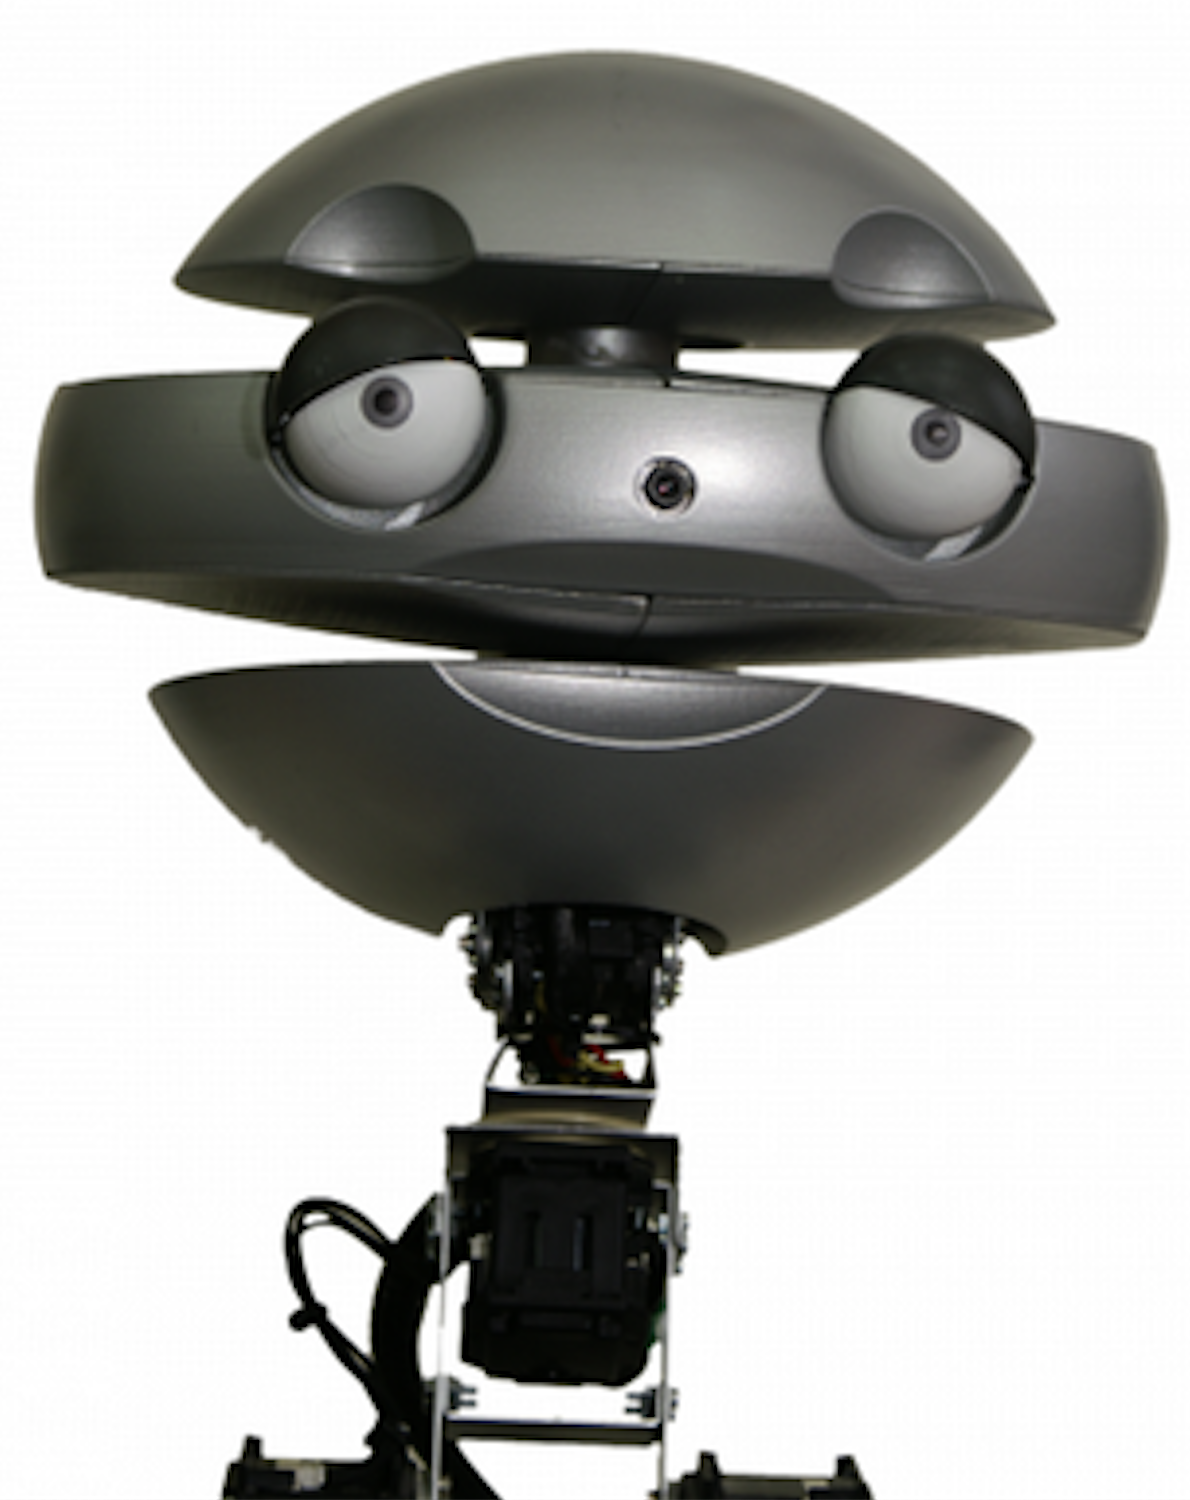
\includegraphics[width=0.4\textwidth]{images/emys.png}
		\caption{EMYS robot.}
		\label{fig:robots:EMYS}
	\end{minipage}
	\hfill
	\begin{minipage}[b]{.4\textwidth}
		\centering
		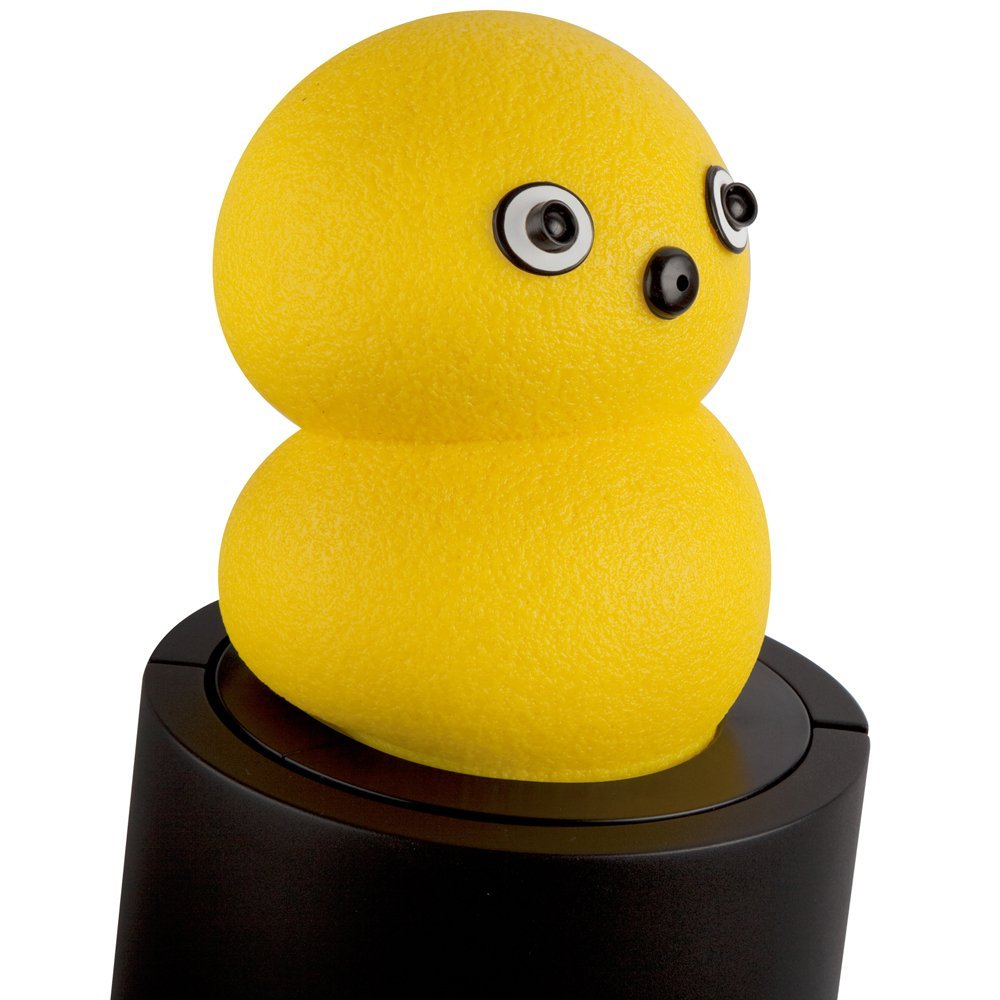
\includegraphics[width=0.4\textwidth]{images/Keepon.jpg}
		\caption{Keepon robot.}
		\label{fig:robots:Keepon}
	\end{minipage}
\end{figure}
%\vspace{-4mm}

\ac{SERA} follows the SAIBA model~\cite{Kopp2006} and is very similar to \ac{ROS}~\cite{Quigley2009} due to, respectively, the separation between intention planning, behaviour planning and realisation, and due to the usage of decoupled modules in an asynchronous messaging system. It aims to be used by both technical and non-technical developers such as psychologists~\cite{Tullio2015}, an advantage as their knowledge is crucial during the development and analysis of \ac{HRI}. For example, utterances are modelled using markup text that can contain non-interrupting behavioural rules and can be developed by non-technical teams.

The most important components are Thalamus, Skene and Nutty Tracks.
\begin{itemize}
	\item \textbf{\textit{Thalamus}}: responsible for receiving and delivering the published messages to the right subscribers;
	\item \textbf{\textit{Skene}}: responsible for translating high-level intentions generated at the decision-making level into a schedule of behaviour actions;
	\item \textbf{\textit{Nutty Tracks}}: responsible for managing animations.
\end{itemize}

\textit{Skene} is the most relevant component in \ac{SERA} for the development of rapport agents as it is the controller that plans animations and non-verbal behaviours such as gaze, utterances and animations according to perceptual messages. This component is rule-based and has an explicit representation of its body position over his physical environment. 

SERA also includes modules for bridging external tools such as \ac{FAtiMA} to model emotions~\cite{Dias2011} or Unity to create virtual scenarios. All these modules co-exist inside the \textit{Thalamus} ``network'' to cooperate, in order to achieve the interactional goals in any \ac{HRI} scenario (e.g., negotiation scenarios on Figure~\ref{fig:SERA:Examples}).

\begin{figure}
	\centering
	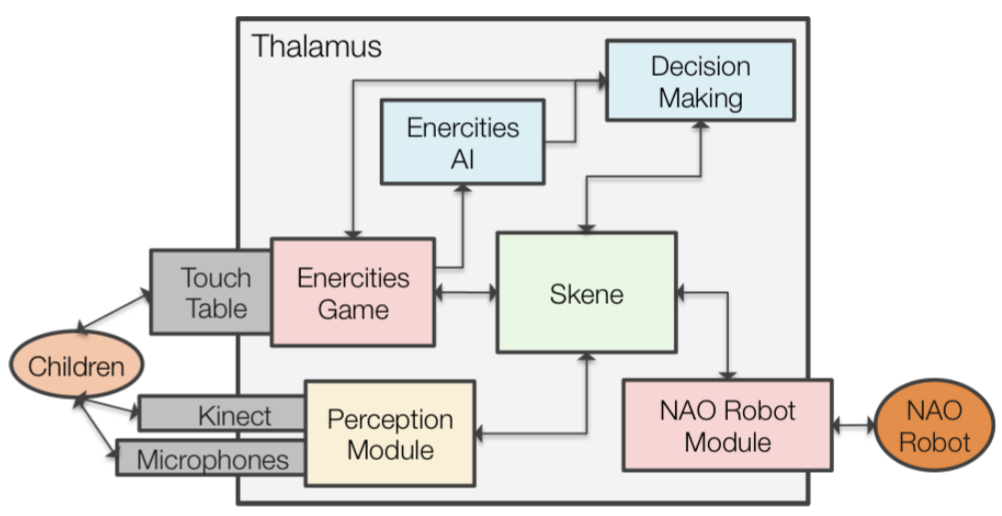
\includegraphics[width=0.6\linewidth]{images/SERA_ExSystemEC.png}
	\caption{Enercities scenario system architecture integrated with SERA framework. From~\cite{Tullio2015}.}
	\label{fig:SERA:Examples}
\end{figure}
%\vspace{-4mm}

Despite being under development, \ac{SERA} is stable and demonstrates its applicability in a wide range of \ac{HRI} scenarios. However, the \textit{Skene} component lacks rapport management strategies and it does not adapt its actions when interrupted by the user, which reduces coordination and the overall feeling of rapport. Moreover, the \textit{Skene} component is rule-based which is not sufficiently elegant to build systems more appealing and natural to end-users.
\subsection{Architecture}
\label{sub:sec:solution:arch}

In order to evaluate the proposed backchannel behaviour generation \ac{ML} classifier we require a robotic rapport agent to be tested on human subjects. We propose extending \ac{SERA} framework to manage rapport by providing tools for stimulating positivity, coordination, and mutual attention (similar to Figure~\ref{table:BuildingRapportPlan} on Section~\ref{subsec:Rapport}) enabling flexibility, and reusability in different scenarios. Despite backchannel behaviours being more targeted to enhance mutual attention and coordination, we intend to stimulate positivity as well, by using specific interactional rules.

The architecture that will instantiate the above proposal is depicted in Figure~\ref{fig:rapport:archicture}. The system decision making process is managed by the \textit{Rapport Controller} Module that contains three components: a rule-based and two \ac{ML}-based components.

\begin{figure}
	\centering
	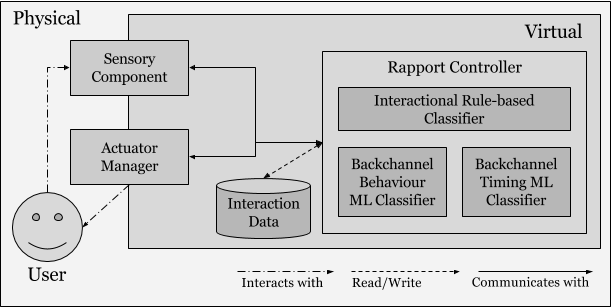
\includegraphics[width=0.75\textwidth]{images/Rapport_archtu.png}
	\caption{Partially decided Rapport Architecture proposal.}
	\label{fig:rapport:archicture}
\end{figure}

The rule-based component is responsible for managing high-level interactional rules that are easier to specify, for example, compliment cooperation actions to stimulate positivity. These rules can be either context specific, or generic enough to be included in other scenarios. The \textit{Interactional Data} data storage depicted in Figure~\ref{fig:rapport:archicture} containts relevant information to manage the interaction.

Two \ac{ML}-based components will handle more complex perceptual states that may arise during the sessions and that would be hard to explicitly define behavioural rules. One module will return correct timings for the generation of backchannels and the other will return the most fitting backchannel behaviour. For example, the first module will suggest that the current instance is appropriate, and the second module will return head nod as the most adequate social behaviour. The retrieved features should be as context independent as possible, including features such as facial expression, head nod frequency, presence of a smile, silence duration, and gaze position. The dominant \ac{ML} classifier is \acf{RL} (Section~\ref{subsec:ReinforcementLearning}) as it was suggested by several authors~\cite{Thomaz2006, Kok2012, Zhao2014, Papangelis2014}.

The \textit{Rapport Controller} will redirect perceptual information collected from the \textit{Sensory Component} and \textit{Actuator Manager} to its component, and will analyse the returned result. From it, the controller will decide which actions should be initiated, maintained or even interrupted. With the bidirectional relationship between the \textit{Rapport Controller}, the \textit{Sensory Component}, and the \textit{Actuator Manager}, we aim to extend \ac{SERA} to support interruptible actions and allow quick adjustments to the agent's behaviour and build better rapport~\cite{Reidsma2011, Visser2014, Kopp2007, Zwiers2011}. For example, similarly to the agent described in Section~\ref{sub:sec:virtualrapport2}, interrupting current speech acts whenever the user starts to speak.

Conflicts may arise between the rule-based component and the \ac{ML}-based components. If the generated behaviours do not conflict with each other, e.g. gaze target and smiling, both actions are executed by the agent. If the generated behaviour conflicts with another, then the \ac{ML}-based components take priority over the rule-based. If there is conflict between two rules, the one with the highest priority takes place (e.g., silence over vocalisation when detecting user's speech).
\subsection{Learning Subconscious Behaviours}
\label{sub:sec:solution:WoZ}

Both \ac{ML}-based modules proposed in Section~\ref{sub:sec:solution:arch} need to be trained in order to learn how to generate correct backchannels. Note, as mention in Section~\ref{subsec:RestrictedPerceptionsWOZStudy}, that in \ac{WoZ} the human subject is not aware that the agent is being controlled manually (partially or fully) by another human, the wizard. In the traditional \ac{WoZ}, the wizards have full access to what is happening in the scenario and have control over the virtual agent, using a \ac{UI}. However, as aforementioned by Sequeira et al., it is relevant to take into account that the virtual agent has inherent limitations in their perceptional abilities and their actions onto their external world~\cite{Sequeira2016}. Moreover, social behaviours are mostly done subconsciously, therefore, the experiment could be influencing the results by just forcing the user to rationalise over what is being subconsciously felt. Taking this two issues into account, we propose an approach for learning correct backchannel generation in virtual agents and embodied agents in \ac{HRI} using limited-perception \ac{WoZ} and human experts for corrective feedback (Figure~\ref{fig:learning:process}).



\begin{figure}
	\centering
	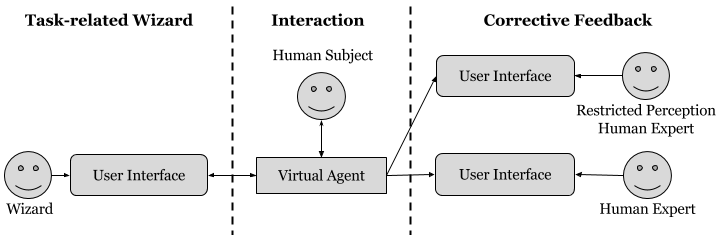
\includegraphics[width=\textwidth]{images/CorrectiveFeedbackRestrictiveWoZ_Diagram.png}
	\caption{Using perceptual readings and limited perception \ac{WoZ} to assess backchannels quality. Human experts monitor the interaction and provide corrective feedback according to their perceptions. The task-related wizard is optional.}
	\label{fig:learning:process}
\end{figure}

Following Figure~\ref{fig:learning:process}, one wizard is responsible for controlling the virtual agents task-related actions and two human experts for providing corrective feedback regarding whether the agent's behaviour is socially appropriate or inappropriate~\cite{Kok2012, Poppe2011}, using a \ac{UI}. One human expert will have its perceptions limited with same extent as the virtual agent, and the other will have unrestricted perceptions. This approach can be seen as reverse-\ac{RL} since it is possible to map the human experts feedback to a reward function, in which, appropriate and inappropriate backchannels will have values values $1$ and $-1$, respectively.

Using this approach it is possible to obtain multiple feedback over the generated behaviours, similar to \ac{PCS}~\cite{Huang2010} without influencing the results by forcing the users to rationalise their actions. Cohen's kappa coefficient $\kappa$ may be used to measure inter-rated agreement between two human experts (Equation~\ref{eq:CohenKappa}). In the equation, $p_0$ is the relative observed agreement and $p_e$ the probability of random agreement.


\vspace{-3mm}
\begin{equation}
	\label{eq:CohenKappa}
	\kappa = \frac{p_0 - p_e}{1 - p_e}
\end{equation}

With the data collected using the restricted-perception \ac{WoZ}, the data will be pre-processed and used to train the \ac{ML}-based component using Weka~\cite{Hall2009}. \ac{RL} algorithms will take priority since they were the main suggestion from several authors~\cite{Thomaz2006, Kok2012, Zhao2014, Papangelis2014, Blumberg2002, Andrist2015, Mutlu2006}. Nevertheless, similar approaches can be further investigated. 

As summarised in equation~\ref{eq:IterativeSolutionEquation}, the system evolves as follows. The initial version $M_0$ is the only version that is strictly rule-based and stripped of previous knowledge according to the information collected from preliminary studies, and the interactional goals. The goal of $M_0$ is to explore as many state combinations as possible in order to produce great number of backchannels, and acquire, as much corrective feedback as possible from the human experts~\cite{Kok2012}. The corrective feedback collected on $M_n$ is later used to train $M_{n+1}$ version of the rapport agent. Following this pattern, we expect $M_n$ to build better rapport than the previous $M_{n-1}$ version. Note that, after the first learning state, the initial excessive backchannels rules must be discarded and replaced by the \ac{ML} generated backchannels, similar to how \ac{IPL} (Section~\ref{subsec:IterativePerceptualLearning}) discards the negative samples after the first subjective evaluations. 

\vspace{-3mm}
\begin{equation}
	\label{eq:IterativeSolutionEquation}
	M_{n+1} = M_{n} + Corrective\, Feedback
\end{equation}

To conclude, after several iterations~\cite{Sequeira2016, Kok2012}, the best possible model $M_n$ will be one tested on users, in which human experts are not required to be present since the agent does not benefit from further training. The final system should represent the average listener's behaviour interacting with the average speaker. Preliminary studies may be conducted to assess the feasibility of the proposed learning strategy.